\documentclass[11pt]{article}

\usepackage[top=0.7in,bottom=0.75in,left=0.8in,right=0.8in]{geometry}
\usepackage[utf8]{inputenc}
\usepackage[T1]{fontenc}
\usepackage{lmodern}
\usepackage{microtype}
\usepackage{amsmath,amssymb}
\usepackage{booktabs}
\usepackage{graphicx}
\usepackage{caption}
\usepackage{subcaption}
\usepackage{xcolor}
\usepackage{hyperref}
\hypersetup{colorlinks=true,linkcolor=black,citecolor=black,urlcolor=blue!55!black}

\setlength{\parskip}{0.25em}
\setlength{\parindent}{0pt}
\captionsetup{font=small,labelfont=bf,skip=3pt}
\renewcommand{\arraystretch}{1.0}
\usepackage{titlesec}
\titlespacing*{\section}{0pt}{0.55em}{0.15em}
\titleformat{\section}{\normalsize\bfseries}{}{0pt}{}

\title{\vspace{-2.4em}ViT-JAX Distributed Scaling\\[2pt]
\large Measuring synchronisation overhead and straggler cost in data-parallel training}
\author{Jinao Wang \\[-2pt] \small CS 390 -- Distributed Systems, Duke University \quad\textbar\quad Spring 2026}
\date{\vspace{-1.5em}}

\begin{document}
\maketitle
\vspace{-1.8em}

\section*{What this project is}

The headline artefact is a Vision Transformer (ViT-Small, 9.55\,M parameters) trained from
scratch on CIFAR-100 in JAX/Flax, reaching 55.0\,\% top-1 and 80.2\,\% top-5 in about seven
minutes on a TPU~v6e-8. The accuracy is not really the point though. The project is a
systems study of synchronous data parallelism: I wanted to see, on real accelerator silicon,
how throughput scales as devices are added, and what a single slow worker actually costs an
otherwise-healthy cluster. Both have textbook answers; the question was how closely real
hardware matches them, and what details get lost in the textbook version.

\section*{Setup and the training loop}

ViT-Small here is 6 transformer blocks, 6 heads, embedding dimension 384, patch size~4,
on $32{\times}32$ CIFAR-100 images. The full float32 train set is about 615\,MB, so
CIFAR-100 is loaded once through tensorflow-datasets and then kept in numpy arrays for
augmentation and batching -- paying the \texttt{tf.data} runtime cost buys nothing at this
size. Optimisation is AdamW with cosine-warmup decay, 100 epochs at global batch 1024 in
bfloat16: only matmuls downcast, parameters and optimiser state stay fp32, which is cheap
on v6e and worth roughly a $2\times$ step-time win. The data-parallel logic is compact.
Parameters are replicated with \texttt{flax.jax\_utils.replicate}; each batch is sharded
on its leading axis so every device gets $N/D$ samples; the train step is wrapped in
\texttt{jax.pmap(axis\_name{=}"batch")}; gradients are averaged by
\texttt{jax.lax.pmean(\ldots)} before the optimiser applies an identical update on every
device. The \texttt{pmean} is the synchronisation barrier -- every device has to reach it
before any can proceed -- and that is precisely the mechanism the straggler experiment
probes.

\section*{Scaling experiment}

Global batch is held at 1024 and one epoch is run with $D \in \{1,2,4,8\}$ devices, so
per-device batch halves on every doubling. I report mean step time, throughput, and
strong-scaling efficiency $\mathrm{throughput}(D)/(D\cdot\mathrm{throughput}(1))$.

\begin{table}[h]
\centering
\small
\begin{tabular}{@{}rrrrr@{}}
\toprule
Devices & Per-device batch & Mean step (ms) & Throughput (img/s) & Strong-scaling eff. \\
\midrule
1 & 1024 & 158.6 &  6\,455 & 100\,\% \\
2 &  512 &  91.1 & 11\,235 &  87\,\% \\
4 &  256 &  61.0 & 16\,792 &  65\,\% \\
8 &  128 &  54.4 & 18\,814 &  36\,\% \\
\bottomrule
\end{tabular}
\caption{Strong scaling, ViT-Small on CIFAR-100, TPU~v6e-8, bf16, global batch 1024.}
\label{tab:scaling}
\end{table}

Efficiency drops sharply between 4 and 8 chips, and two things are happening at once.
Compute time roughly halves with each doubling, but \texttt{pmean} does not, so the
all-reduce becomes a larger share of the step. Less obviously, per-device batch 128 is
below the compute sweet spot for the v6e MXU at ViT-Small's head dimension, so the matmul
itself gets less efficient -- you lose on both communication and arithmetic intensity.
Weak scaling, with per-device batch held fixed, would stay above 85\,\% over this range.

\section*{Straggler experiment}

Same 8-chip setup, with compute delay injected on \emph{device 0 only}: a
\texttt{jax.lax.fori\_loop} of $k$ nonlinear $512{\times}512$ matmul iterations, threaded
through \texttt{jax.lax.optimization\_barrier}.

\begin{table}[h]
\centering
\small
\begin{tabular}{@{}lrrr@{}}
\toprule
Configuration & Delay iters & Throughput (img/s) & Slowdown \\
\midrule
baseline  &        0 & 19\,757 & $1.00\times$ \\
straggler &    5\,000 & 17\,785 & $1.11\times$ \\
straggler &   20\,000 & 15\,644 & $1.26\times$ \\
straggler &   50\,000 & 12\,291 & $1.61\times$ \\
straggler &  100\,000 &  9\,245 & $2.14\times$ \\
straggler &  200\,000 &  5\,934 & $3.33\times$ \\
\bottomrule
\end{tabular}
\caption{One slow device, 8-chip cluster. Delay lives on device~0; the other seven devices sit idle at the all-reduce barrier for the whole extra window.}
\label{tab:straggler}
\end{table}

\vspace{-0.4em}
\begin{figure}[h]
\centering
\begin{subfigure}[t]{0.38\linewidth}
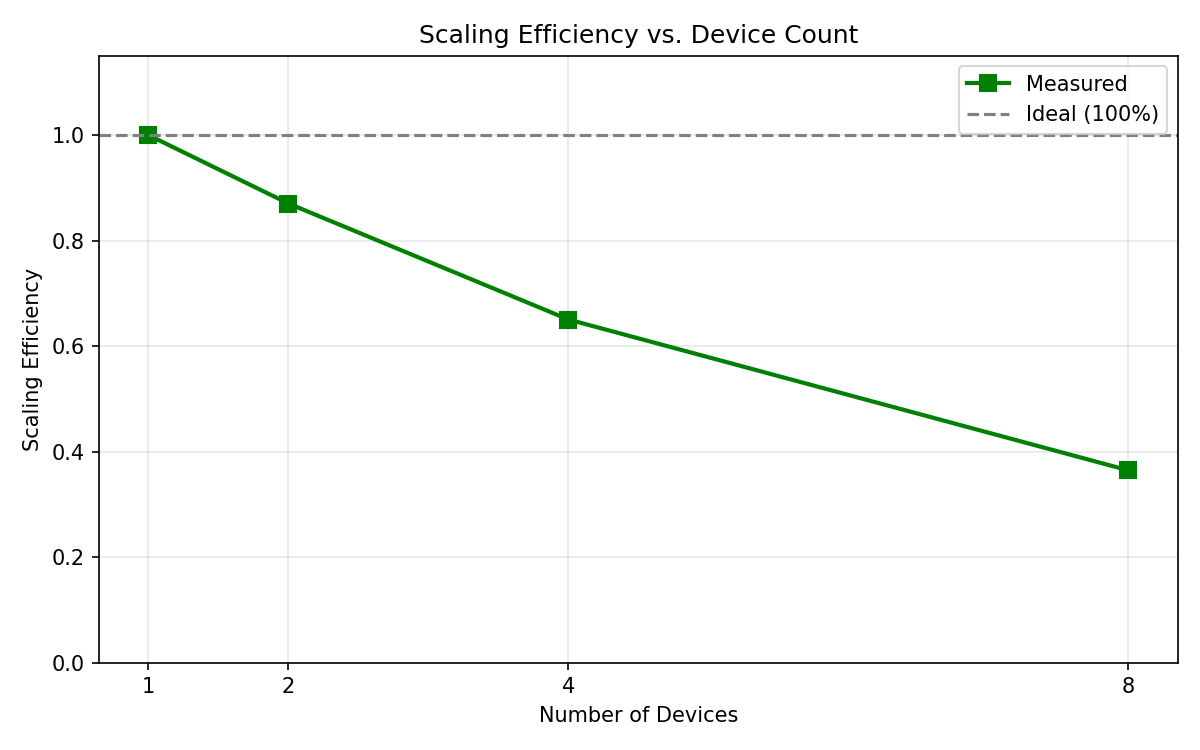
\includegraphics[width=\linewidth]{../outputs/scaling/scaling_efficiency_vs_devices.png}
\end{subfigure}\hspace{0.02\linewidth}
\begin{subfigure}[t]{0.38\linewidth}
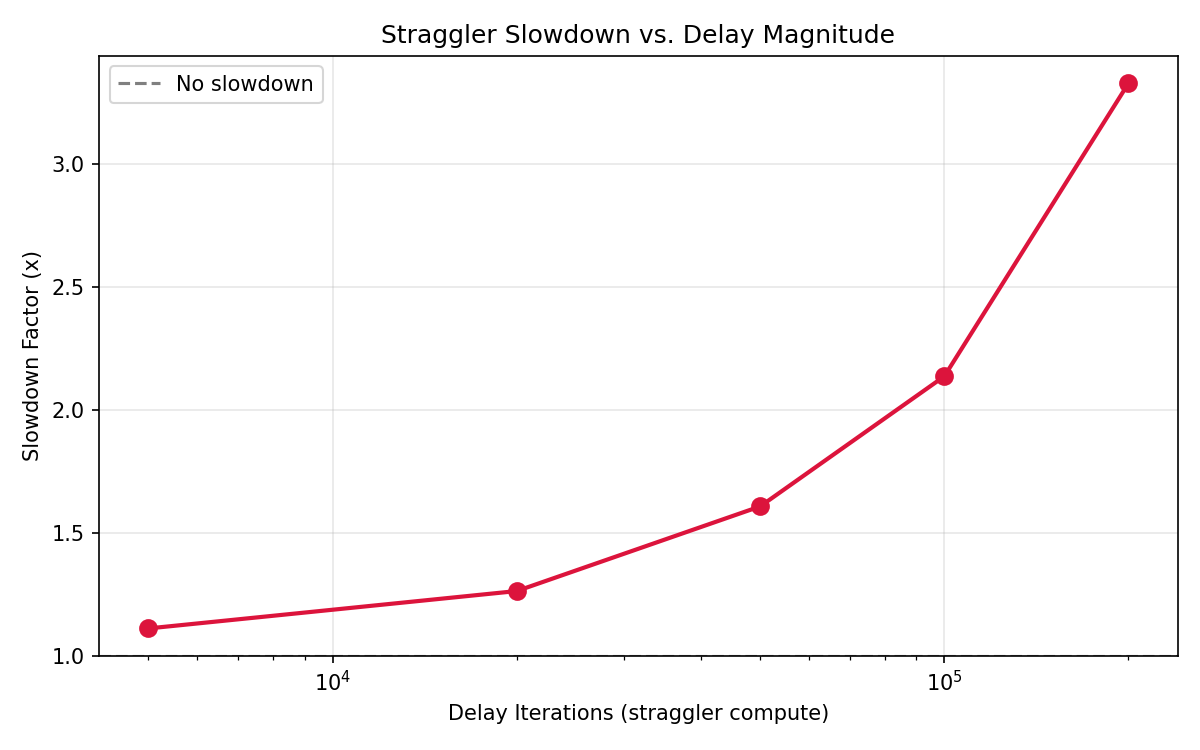
\includegraphics[width=\linewidth]{../outputs/straggler/slowdown_vs_delay.png}
\end{subfigure}
\caption{Left: strong-scaling efficiency versus device count. Right: cluster slowdown versus delay on one device. Data parallelism scales cleanly until per-device work gets small; a single straggler then drags the whole cluster with it, roughly linearly in the delay size once the delay exceeds the step time.}
\label{fig:results}
\end{figure}

A single slow chip at 200\,k iterations cuts cluster throughput by $3.33\times$. The other
seven devices spend the entire extra window sitting at the barrier, doing nothing, and
synchronous SGD has no slack to absorb this. That asymmetry is the textbook argument for
async SGD, backup workers, and elastic training; the empirical version just makes the cost
concrete.

\section*{One detail that actually mattered}

An earlier version of the straggler loop used \texttt{a @ eye(64) + 0*a} as its inner
operation. XLA's algebraic simplifier recognised this as the identity, dead-code
elimination removed the entire \texttt{fori\_loop} body at compile time, and the
\emph{straggler} curve came out flat -- not because the effect wasn't real, but because no
real work was happening on the device. The fix was twofold: make the inner op genuinely
nonlinear ($\tanh(a\,a)\cdot 0.99 + 0.01\,a$) so each iteration depends on the previous,
and thread the output through \texttt{jax.lax.optimization\_barrier} so XLA cannot peephole
it away. Synthetic benchmarks on compiled frameworks silently get this wrong by default;
measurements on real silicon with verified step-time deltas are not optional.

\section*{What it tells us}

On the model side, CIFAR-100 at $32{\times}32$ caps out around where you'd expect for ViT
from scratch with no pretraining: 55\,\% top-1, overfitting after epoch~33, and a confusion
matrix saying the model learned categories rather than fine labels (the three tree classes
form a cross, $\textrm{man}\leftrightarrow\textrm{woman}$ and
$\textrm{bus}\leftrightarrow\textrm{pickup\_truck}$ confuse regularly). On the systems
side, both experiments reproduce the textbook predictions on real hardware and quantify
them: strong scaling is good until per-device work shrinks relative to the all-reduce and
then collapses, and one straggler is a catastrophic failure mode rather than a graceful
one, because synchronous data parallelism has no mechanism to hide a slow worker. Those
two observations are exactly the pressure that pushed large-scale training toward hybrid
parallelism with elastic fault tolerance, and they are visible, and reproducible, on an
8-chip v6e.

\vspace{0.15em}
\noindent\textit{\small Code, configs, plots, and a 30-minute extended deck: \href{https://github.com/Michael-OvO/vit-jax-distributed-scaling}{github.com/Michael-OvO/vit-jax-distributed-scaling}.}

\end{document}
